\scanpage{160}
\deleted{
\uline{1.1.84}

Compléments et rectifications sur les facettes exceptionnelles de $(\unsure{X|\mathcal X},K)$

a) Avec les notations de \unsure{i)}, on a
\[
\varphi^{-1}(\unsure{X_1^a|X_1^0})=L\cup K_0\qquad(\text{et non }=L\,!)
\]

b) La structure d'une facette exceptionnelle au voisinage d'une arête exceptionnelle (ou mieux, de la \inserted{double} paire de facettes rattachées à un sommet exceptionnel $a$) est de la forme suivante :
\figure{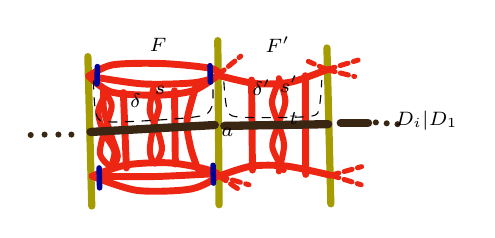
\begin{tikzpicture}[x=.55cm,y=-.55cm,line cap=round,line join=round,g/.style={olive!80!yellow,line width=1.7pt},r/.style={orange!80!brown,line width=1.8pt},w/.style={red!60!black,line width=1.5pt},b/.style={blue!60!black,line width=1.4pt},p/.style={gray!70,thin},k/.style={black,line width=1.2pt},every node/.style={font=\scriptsize}]
\draw[g,line width=2.6pt] plot[smooth] coordinates {(2.98,11.4) (3.07,14.85)};
\draw[g,line width=2.6pt] plot[smooth] coordinates {(5.98,11.03) (6.01,14.82)};
\draw[g,line width=2.6pt] plot[smooth] coordinates {(8.5,11.2) (8.59,14.8)};
\draw[red!70!brown,line width=2.5pt] plot[smooth] coordinates {(3.0,11.85) (3.55,11.59) (4.7,11.56) (5.81,11.67) (5.98,11.83) (5.46,12.0) (4.25,12.03) (3.0,11.85)};
\draw[red!70!brown,line width=2.5pt] plot[smooth] coordinates {(3.0,11.85) (3.53,12.22) (4.62,12.29) (5.43,12.18) (5.98,11.83)};
\draw[red!70!brown,line width=2.5pt] plot[smooth] coordinates {(3.08,14.16) (3.88,13.9) (4.95,13.86) (5.96,14.1) (5.39,14.45) (4.12,14.49) (3.08,14.16)};
\draw[red!70!brown,line width=2.5pt] plot[smooth] coordinates {(3.08,14.16) (4.5,14.17) (5.96,14.1)};
\draw[red!70!brown,line width=2.5pt] plot[smooth] coordinates {(5.98,11.83) (6.84,12.02) (7.66,11.99) (8.5,11.7)};
\draw[red!70!brown,line width=2.5pt] plot[smooth] coordinates {(6.01,14.16) (6.75,13.93) (7.58,13.93) (8.59,14.14)};
\draw[red!70!brown,line width=2.5pt] plot[smooth] coordinates {(3.8,12.23) (3.87,13.97)};
\draw[red!70!brown,line width=2.5pt] plot[smooth] coordinates {(4.98,12.19) (5.0,13.88)};
\draw[red!70!brown,line width=2.5pt] plot[smooth] coordinates {(5.47,12.11) (5.27,12.88) (5.35,13.49) (5.51,13.98)};
\draw[red!70!brown,line width=2.5pt] plot[smooth] coordinates {(6.76,11.94) (6.78,14.02)};
\draw[red!70!brown,line width=2.5pt] plot[smooth] coordinates {(8.0,11.84) (8.01,14.12)};
\draw[red!70!brown,line width=2.2pt] plot[smooth] coordinates {(3.33,12.16) (3.53,12.53) (3.36,13.11) (3.26,13.65) (3.51,13.93) (3.67,13.7) (3.51,13.19) (3.36,12.69) (3.33,12.16)};
\draw[red!70!brown,line width=2.2pt] plot[smooth] coordinates {(3.42,12.21) (3.22,12.65) (3.33,13.12) (3.59,13.58) (3.51,13.95)};
\draw[red!70!brown,line width=2.2pt] plot[smooth] coordinates {(4.49,12.15) (4.62,12.55) (4.49,13.02) (4.41,13.58) (4.53,13.87) (4.69,13.55) (4.6,13.13) (4.41,12.66) (4.49,12.15)};
\draw[red!70!brown,line width=2.2pt] plot[smooth] coordinates {(7.39,11.9) (7.54,12.43) (7.37,12.98) (7.24,13.49) (7.5,14.02)};
\draw[red!70!brown,line width=2.2pt] plot[smooth] coordinates {(7.4,11.95) (7.23,12.45) (7.39,12.98) (7.51,13.45) (7.39,14.05)};
\draw[red!70!brown,densely dashed,line width=1.8pt] plot[smooth] coordinates {(5.98,11.83) (6.51,11.39)};
\draw[red!70!brown,densely dashed,line width=1.8pt] plot[smooth] coordinates {(8.5,11.7) (8.07,11.51)};
\draw[red!70!brown,densely dashed,line width=1.8pt] plot[smooth] coordinates {(8.5,11.7) (9.22,11.48)};
\draw[red!70!brown,densely dashed,line width=1.8pt] plot[smooth] coordinates {(8.5,11.7) (9.14,11.86)};
\draw[red!70!brown,densely dashed,line width=1.8pt] plot[smooth] coordinates {(6.01,14.16) (6.7,14.36)};
\draw[red!70!brown,densely dashed,line width=1.8pt] plot[smooth] coordinates {(6.01,14.16) (6.44,14.45)};
\draw[red!70!brown,densely dashed,line width=1.8pt] plot[smooth] coordinates {(8.59,14.14) (9.3,13.94)};
\draw[red!70!brown,densely dashed,line width=1.8pt] plot[smooth] coordinates {(8.59,14.14) (9.29,14.36)};
\draw[k,dashed,thin] plot[smooth] coordinates {(3.11,11.96) (3.18,12.75) (3.55,12.91) (5.47,12.79) (5.84,12.56) (5.86,11.94)};
\draw[k,dashed,thin] plot[smooth] coordinates {(6.12,11.98) (6.21,12.66) (6.55,12.8) (8.1,12.78) (8.32,12.57) (8.38,11.95)};
\draw[black!70!brown,line width=3pt] plot[smooth] coordinates {(3.04,13.14) (5.91,12.98)};
\draw[black!70!brown,line width=3pt] plot[smooth] coordinates {(6.13,13.0) (8.53,12.96)};
\draw[black!70!brown,line width=3pt] plot[smooth] coordinates {(8.82,12.93) (9.45,12.93)};
\fill[black!70!brown] (1.66,13.21) circle (.07);
\fill[black!70!brown] (1.98,13.2) circle (.07);
\fill[black!70!brown] (2.3,13.2) circle (.07);
\fill[black!70!brown] (2.6,13.2) circle (.07);
\fill[black!70!brown] (9.63,12.92) circle (.07);
\fill[black!70!brown] (9.88,12.94) circle (.07);
\fill[black!70!brown] (10.13,12.96) circle (.07);
\draw[blue!60!black,line width=2pt] plot[smooth] coordinates {(3.2,11.63) (3.19,12.03)};
\draw[blue!60!black,line width=2pt] plot[smooth] coordinates {(5.8,11.61) (5.81,11.99)};
\draw[blue!60!black,line width=2pt] plot[smooth] coordinates {(3.24,13.97) (3.25,14.43)};
\draw[blue!60!black,line width=2pt] plot[smooth] coordinates {(5.87,13.91) (5.88,14.32)};
\node at (4.6,11.13) {$F$};
\node at (7.36,11.13) {$F'$};
\node at (4.08,12.43) {$\delta$};
\node at (6.99,12.12) {$\delta'$};
\node at (4.65,12.17) {$\unsure{s}$};
\node at (7.62,12.04) {$\unsure{s'}$};
\node at (10.8,12.87) {$\unsure{D_i|D_1}$};
\node at (6.2,13.14) {$\unsure{a}$};
\node at (7.73,12.84) {$\unsure{t}$};
\end{tikzpicture}}

Choix d'une \unsure{la} ``branche principale'' \inserted{$\delta$} de $L$ dans une face exceptionnelle ($F$ ou $F'$ disons) en un sommet \deleted{multiple}\inserted{multiple $s$}; alors les branches de $L$ en $s$ distinctes de \deleted{$\unsure{\delta}$} $\delta$ sont concourantes en un m\textsuperscript{me} pt $\unsure{t}$ de $\partial F$ sur $K_0$ (et par la loi de symétrie, le m\textsuperscript{me} doit se faire avec m\textsuperscript{me} multiplicité.

(De plus, je rappelle que la loi de symétrie s'étend à la multiplicité des \unsure{pts demi sommets|pts deux sommets} \deleted{\unsure{multiples}} \inserted{de $L$} qui se trouvent sur les deux arêtes ordinaires, incidentes à $a$.)

c) Pour les arêtes de $F$ \inserted{\unsure{non exceptionnelles en $F$}} distinctes des trois arêtes marquées, \deleted{\unsure{la}} la \deleted{bord} rive privilégiée est celle opposée à cette face. -- pour une arête \inserted{ordinaire} passant par un sommet exceptionnel (arête marquée en vert), la \deleted{arête}\inserted{rive} privilégiée est celle qui correspond à la face \unsure{instble}.

d) Pour avoir la position relative correspondant à une face exceptionnelle, il faut modifier le \unsure{ruban généralisé} \deleted{\unsure{(disons}} (dis. $A$ qui \unsure{prend} $\varphi(\partial F^*)$, où $F^*$ est déduite de $F$ par renflement \unsure{en} les sommets critiques dans la rive \deleted{\unsure{exceptionelle}} privilégiée et opposée à $F$) en \deleted{\unsure{faisant une}}\inserted{déformant $F^*$ de} façon similaire, à partir de la modification obtenue en remplaçant ``\uuline{l'arc} \deleted{\unsure{des deux pts exceptionnels de}} \inserted{\unsure{du bord}} exceptionnel'' \deleted{de la}\inserted{de la} face envisagée (joignant les deux pts critiques principaux \deleted{sur la} face) par un ``\unsure{path}'' parallèle à l'intérieur de $F$ (cf. pointillé au stylo).
}
\margin{\mspage{159}}
